%----------------------------------------------------------------------------------------
%	CHAPTER 7
%----------------------------------------------------------------------------------------
\chapterimage{ChapterImages/chapter7.png} % Chapter heading image

\chapter{Shell Programming III}
\label{ch:shell3}

With variables, conditionals, and loops from Chapters~\ref{ch:shell1} and~\ref{ch:shell2}, you already have everything needed to write working scripts. The last piece is \textbf{functions} -- a way to package a block of logic under a name, so it can be reused instead of copy-pasted, and so a long script can be organized into clear, testable pieces.

\section{What Is a Function?}
A function is a named block of code that performs a specific task. It allows you to reuse logic, reduce redundancy, and organize scripts into smaller, manageable parts.

\textbf{Advantages:}
\begin{itemize}
    \item Reuse code instead of rewriting it.
    \item Simplify debugging and maintenance.
    \item Improve script readability and structure.
\end{itemize}

\section{Defining Functions}
Functions in Bash can be declared in two equivalent ways:
\begin{lstlisting}[language=Terminal]
#!/bin/bash
# With the function keyword
function greet() {
    echo "Hello, $1!"
}

# Without the function keyword
greet() {
    echo "Hello, $1!"
}
\end{lstlisting}
There is \textbf{no need} to declare argument types or the number of arguments -- unlike C or Python, Bash functions accept any number of arguments of any type (everything is treated as text).

\section{Calling Functions}
To execute a function, call it by its name followed by any arguments, exactly as you would call any other command:
\begin{lstlisting}[language=Terminal]
greet "Ali"
\end{lstlisting}

\textbf{Syntax:}
\begin{lstlisting}[language=Terminal]
function_name arg1 arg2 ...
\end{lstlisting}
\textbf{Important:} a function must be \emph{defined} before it is called -- Bash reads the script top to bottom, so calling a function above its definition fails.

\section{Function Arguments}
Function arguments are accessed using positional parameters, the same special variables also used for script arguments:

\begin{table}[h!]
\centering
\small
\renewcommand{\arraystretch}{1.3}
\begin{tabular}{|>{\centering\arraybackslash}p{3cm}|>{\raggedright\arraybackslash}p{9cm}|}
\hline
\textbf{Symbol} & \textbf{Meaning} \\ \hline
\texttt{\textdollar0} & Script name \\ \hline
\texttt{\textdollar1, \textdollar2, \textdollar3, ...} & Function arguments, by position \\ \hline
\texttt{\textdollar\#} & Number of arguments \\ \hline
\texttt{\textdollar@} & All arguments, as separate words \\ \hline
\end{tabular}
\caption{Special Variables in Shell Scripting}
\label{tab:special-vars}
\end{table}

Figure~\ref{fig:function-anatomy} shows how these map onto an actual function call.

\begin{figure}[h]
    \centering
    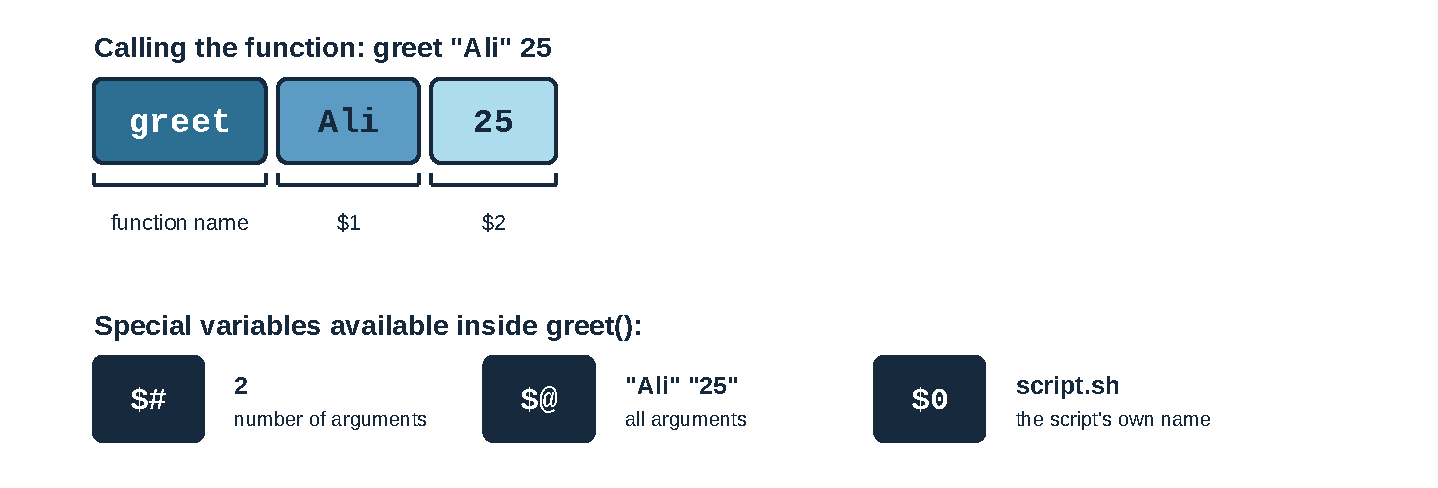
\includegraphics[width=0.95\textwidth]{Images/Chapter7/function-anatomy.pdf}
    \caption{How positional parameters map onto the arguments of a function call.}
    \label{fig:function-anatomy}
\end{figure}

\textbf{Example:}
\begin{lstlisting}[language=Terminal]
#!/bin/bash
print_args() {
    echo "Number of arguments: $#"
    echo "All arguments: $@"
}
print_args 1 2 3
\end{lstlisting}

\section{Returning Values}
Functions in Bash \textbf{do not} return values the way functions do in C or Python. There are two common ways to get a result out of a function instead:

\begin{enumerate}
    \item \textbf{Using \texttt{return} (for an exit status only):} \texttt{return} can only report a small integer (0--255), conventionally used to signal success (\texttt{0}) or failure (any non-zero value) -- not to hand back a computed value.
\begin{lstlisting}[language=Terminal]
#!/bin/bash
check_even() {
    if (( $1 % 2 == 0 )); then
        return 0
    else
        return 1
    fi
}

check_even 4
echo "Exit status: $?"   # 0 -> even
\end{lstlisting}

    \item \textbf{Using \texttt{echo} (to send actual output):} to get a real value -- a number, a string, anything -- have the function \texttt{echo} it, and capture that output with command substitution:
\begin{lstlisting}[language=Terminal]
#!/bin/bash
square() {
    echo $(($1 * $1))
}

result=$(square 4)
echo "Result: $result"
\end{lstlisting}
\end{enumerate}

\section{Variable Scope}
Variables inside a function are \textbf{global by default} -- a function can freely read and overwrite a variable defined outside it. Use the \texttt{local} keyword to limit a variable's scope to that function only, so it doesn't leak out or clash with a variable of the same name elsewhere in the script. Figure~\ref{fig:variable-scope} illustrates this with the example below.

\textbf{Example:}
\begin{lstlisting}[language=Terminal]
#!/bin/bash
my_var="global"

change_var() {
    local my_var="changed inside function"
    echo $my_var
}

change_var
echo $my_var
\end{lstlisting}

\textbf{Output:}
\begin{lstlisting}[language=Terminal]
changed inside function
global
\end{lstlisting}

\begin{figure}[h]
    \centering
    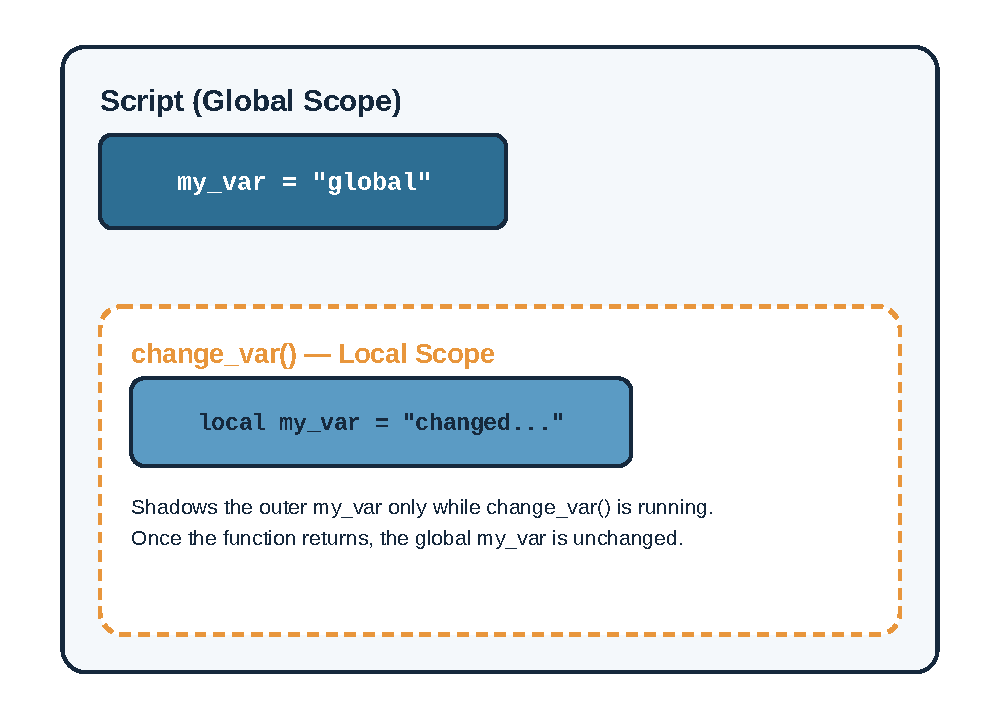
\includegraphics[width=0.8\textwidth]{Images/Chapter7/variable-scope.pdf}
    \caption{A \texttt{local} variable only shadows the global one for the duration of the function call.}
    \label{fig:variable-scope}
\end{figure}

\textbf{Note:} had \texttt{local} been omitted on line~2 of \texttt{change\_var}, the assignment would have overwritten the global \texttt{my\_var}, and the final \texttt{echo \$my\_var} would print \texttt{"changed inside function"} instead of \texttt{"global"}.

\section{Recursive Functions}
Because a Bash function is just a named command, it is allowed to call \emph{itself} -- this is called \textbf{recursion}. A recursive function needs two things to terminate correctly:
\begin{itemize}
    \item A \textbf{base case}: a condition simple enough to answer directly, without another call.
    \item A \textbf{recursive case}: the function calls itself with an input that moves \emph{closer} to the base case.
\end{itemize}
Without a base case (or if the input never actually approaches it), the function calls itself forever until Bash runs out of resources.

\textbf{Example: summing 1 to \texttt{n} recursively}
\begin{lstlisting}[language=Terminal]
#!/bin/bash
sum_to() {
    local n=$1
    if (( n <= 1 )); then
        echo 1              # base case
    else
        local rest=$(sum_to $((n - 1)))   # recursive case
        echo $((n + rest))
    fi
}

echo "Sum: $(sum_to 5)"     # Sum: 15
\end{lstlisting}
\textbf{Explanation:} \texttt{sum\_to 5} calls \texttt{sum\_to 4}, which calls \texttt{sum\_to 3}, and so on down to \texttt{sum\_to 1} -- the base case, which returns \texttt{1} directly. Each call then adds its own \texttt{n} to the result of the call below it, unwinding back up to the original call.

%----------------------------------------------------------------------------------------
%	CHAPTER 7 - HANDS-ON PRACTICES (append at the end of chapter7.tex)
%----------------------------------------------------------------------------------------

\section{Hands-on Practices}
Complete the following three practices using the Linux terminal. Record the commands you use, save your scripts, and explain the results where requested. Work inside your \texttt{os-lab/} directory.

\subsection{Practice 1: Defining, Calling, and Passing Arguments to Functions}
This practice covers the two ways of defining a function, calling a function, the rule that a function must be defined before it is called, and positional parameters.

\begin{enumerate}
    \item Create a directory named \texttt{chapter7-practice} and move into it. Create a script named \texttt{functions.sh} that defines one function named \texttt{greet} using the \texttt{function} keyword and another function named \texttt{greet2} without it. Both should print \texttt{Hello, \$1!}. Call each of them with a different name, make the script executable, and run it. Then move one of the calls above its function definition, run the script again, observe the error, and fix it.
    \item Create a script named \texttt{args.sh} that defines a function \texttt{print\_args} printing the number of arguments (\texttt{\$\#}), all arguments (\texttt{\$@}), and the first two arguments (\texttt{\$1} and \texttt{\$2}). Call it with the arguments \texttt{1 2 3}, then with the words \texttt{red green blue yellow}, and finally with no arguments at all.
    \item Add a function named \texttt{list\_args} to \texttt{args.sh} that uses a \texttt{for} loop over \texttt{"\$@"} to print every argument on its own line in the form \texttt{Argument 1: red}, using a counter variable. Call it with at least four arguments.
\end{enumerate}

Now, answer the following questions:
\begin{itemize}
    \item What are the two ways of declaring a function, and do you need to declare the number or type of its arguments?
    \item What error did you get when you called a function before its definition, and why does Bash behave this way?
    \item What did \texttt{\$\#}, \texttt{\$1}, and \texttt{\$2} contain when \texttt{print\_args} was called with no arguments?
\end{itemize}

\subsection{Practice 2: Returning Values from Functions}
This practice covers returning an exit status with \texttt{return}, returning a real value with \texttt{echo} and command substitution, and using functions together with conditions and loops.

\begin{enumerate}
    \item Create a script named \texttt{status.sh} that defines a function \texttt{check\_even}, which returns \texttt{0} if its first argument is even and \texttt{1} otherwise, using \texttt{(( ))}. Call it with \texttt{4} and with \texttt{7} and print \texttt{\$?} after each call. Then use the function directly as the condition of an \texttt{if} statement to print whether \texttt{10} is even or odd. Finally, add a function that executes \texttt{return 300}, call it, and print \texttt{\$?}.
    \item Create a script named \texttt{values.sh} that defines a function \texttt{square}, which prints the square of its first argument, and a function \texttt{add}, which prints the sum of its two arguments. Capture their output in variables using command substitution and print the results with messages such as \texttt{Result: 16}.
    \item Add a function named \texttt{max} to \texttt{values.sh} that prints the larger of its two arguments. Create an array \texttt{numbers} with at least six numbers, then use a \texttt{for} loop and the \texttt{max} function to find the largest number in the array, and print it.
\end{enumerate}

Now, answer the following questions:
\begin{itemize}
    \item What did \texttt{\$?} contain after \texttt{return 300}, and what does this tell you about using \texttt{return} to send back computed values?
    \item Why can a function be used directly as the condition of an \texttt{if} statement?
    \item Which way of returning values did you use in \texttt{square}, \texttt{add}, and \texttt{max}, and why?
\end{itemize}

\subsection{Practice 3: Variable Scope and Recursive Functions}
This practice covers global and \texttt{local} variables, and recursive functions with a base case and a recursive case.

\begin{enumerate}
    \item Create a script named \texttt{scope.sh} that sets a global variable \texttt{my\_var="global"} and defines two functions: \texttt{change\_global}, which assigns a new value to \texttt{my\_var} without \texttt{local}, and \texttt{change\_local}, which assigns a new value to \texttt{my\_var} using \texttt{local}. Print \texttt{my\_var} before any call, after calling \texttt{change\_local}, and after calling \texttt{change\_global}, and compare the three values.
    \item Create a script named \texttt{recursion.sh} that defines a recursive function \texttt{sum\_to} that calculates the sum of the numbers from $1$ to \texttt{n}, using \texttt{local} variables. Print the result for $5$ and for $10$.
    \item Add a recursive function named \texttt{factorial} to \texttt{recursion.sh}, with a base case for $n \le 1$ and a recursive case that multiplies \texttt{n} by the factorial of \texttt{n - 1}. Use a \texttt{for} loop over \texttt{\{1..6\}} to print the factorial of every number in the range.
\end{enumerate}

Now, answer the following questions:
\begin{itemize}
    \item What is the value of \texttt{my\_var} after each call, and which keyword caused the difference?
    \item What are the base case and the recursive case of your \texttt{factorial} function?
    \item What would happen if a recursive function had no base case, or if its input never moved closer to the base case?
\end{itemize}